\chapter{Problem description} \label{chap:problem_description}

This chapter introduces the optimization problem addressed in this thesis. Section~\ref{sec:competition_overview} provides a brief overview of the competition setting where the problem was initially assigned. In Section~\ref{sec:original_problem_statement}, the original problem statement is presented and explained in detail.
Section~\ref{sec:preprocessing} explains preprocessing steps that we apply to simplify the problem for optimization.
Section~\ref{sec:datasets} describes the datasets provided with the problem. Finally, Section~\ref{sec:simulator} presents the custom simulator tool that we developed to evaluate solutions to the problem.

\section{Competition overview} \label{sec:competition_overview}

The problem we address in this thesis was originally assigned in the qualifying round of Google Hash Code 2021. Google Hash Code was a global team programming competition, running between 2014--2022, where teams of 2--4 competitors solved an optimization problem with the goal of achieving the best score in a limited time of 4 hours. Despite its discontinuation, the competition remains a valuable resource for a wide range of optimization problems and has been the subject of various follow-up studies and articles~\cite{rodrigues2023principled, li2022building}.

The usual solution procedure for our problem was as follows: Read the input data, create a trivial solution and write it to the output file in the specified format, and upload the solution to the evaluation system. The evaluation system not only displayed the score, but also some informative statistics, such as the number of cars that reached the finish before the deadline, the cars that arrived earliest and latest, the average cycle length of traffic lights at intersections, etc.
For some datasets, an interactive visualization of the evaluation process was also available, allowing to see the structure of a particular dataset. Although a local simulator was not needed to solve the problem, the manual upload of the solution to the evaluation system was slow and cumbersome and therefore not suitable for the use of efficient optimization algorithms.

Most teams were able to construct trivial solutions, which they then tried to improve by randomly changing the values. However, the best teams were able to write their own local simulator and use it to run multiple heuristics to get a better total score. Still, there was no time for anything more complex than a simple random search.

The total score was the sum of the scores of all 6 datasets (A--F). The first dataset (A) served as a ``toy problem'' mainly for debugging purposes, but the rest of the datasets were large enough for optimization. It should be noted that the distribution of points among the datasets is uneven, so the contestants mostly focused on the datasets with the highest possible score (D, F) and pragmatically skipped optimizing the rest (B, C, E).

\section{Original problem statement} \label{sec:original_problem_statement}

The full problem statement\footnote{\url{https://github.com/google/coding-competitions-archive/blob/main/hashcode/hashcode_2021_qualification_round.pdf}} is available in the Google Coding Competitions archive~\cite{google2023google}. Here we describe only the parts that are important for understanding this work.
In short, the task is as follows:
\begin{quote}
    \textit{Given a city plan describing intersections and streets and cars with planned paths through the city, optimize the schedule of traffic lights to minimize the total amount of time spent in traffic, and help as many cars as possible reach their destination before a specified deadline.}
\end{quote}
In terms of graph theory, the city plan is a \textit{directed graph}. The intersections are \textit{vertices} and the streets are \textit{directed edges} (see Figure~\ref{fig:hashcode_city_plan}). The planned path for each car is indeed a \textit{path} in this graph because it has a different start and end, and no intersection is repeated.

\begin{figure}
    \centering
    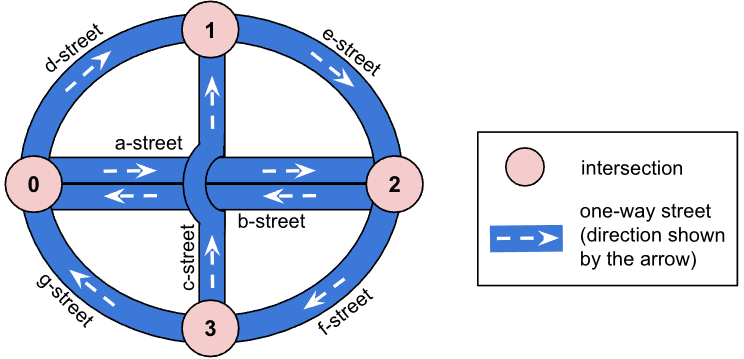
\includegraphics[width=\linewidth]{img/hashcode/figure1.png}
    %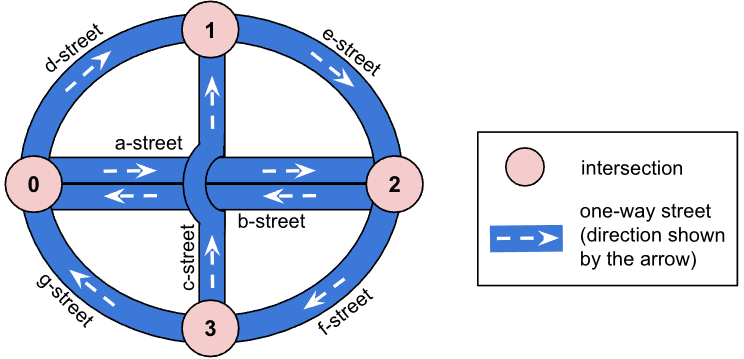
\includegraphics[width=.8\linewidth]{img/hashcode/figure1.png}
    \caption[Example of a city plan]{
        Example of a city plan \cite{google2023google}.
    }
    \label{fig:hashcode_city_plan}
\end{figure}

\subsection{Streets and intersections}

In the city, we have a set of intersections
$I$, where $\abs{I} \in [2, 10^5]$,
and a set of streets
$S \subseteq \{(u, v) | u,v \in I \land u \neq v\}$, where $\abs{S} \in [2, 10^5]$.
Each street $s \in S$ is a unique one-way connection between two different intersections $u$, $v$; two distinct streets $(u, v)$ and $(v, u)$ in opposite directions between the same two intersections are allowed. Each street $s \in S$ has a fixed time $l(s) \in \mathbb{N}_+$ that it takes a car to get from the beginning to the end of the street, independently of the other cars on the street.
Each intersection $i \in I$ has a set of incoming streets $S_i^+ \subset S$, where $\abs{S_i^+} \geq 1$, and a set of outgoing streets $S_i^- \subset S$, where $\abs{S_i^-} \geq 1$; thus each intersection has at least one incoming street and at least one outgoing street.

\subsection{Traffic lights and schedules}

In each intersection $i \in I$, there is a traffic light at the end of each \textit{incoming} street $s^+ \in S_i^+$. The traffic light has two states---green and red. Green means the cars from this street can pass through the intersection and continue to any \textit{outgoing} street $s^- \in S_i^-$ in their path. Red means the cars must stop until the light turns green again. At most one traffic light can be green at each intersection at any time.

When the light is red, cars arriving at the end of a street queue up and wait for the light to turn green. The queue does not take up any space and does not change the distance cars have to travel. When the light is green, one car can pass through an intersection every second. Passing through an intersection, i.e., moving from the end of an incoming street to the beginning of an outgoing street, takes no additional time.

For each intersection $i \in I$, we can set a traffic light schedule. This schedule determines the order and duration of green light for the incoming streets of the intersection. The schedule repeats in a cycle until the end of the simulation (see Figure~\ref{fig:hashcode_traffic_lights}). Each street can appear at most once in the schedule. If a street is not included in the schedule, it is red the whole time, and any waiting cars are blocked. By default, intersections have no schedule and all streets are red.

% https://tex.stackexchange.com/questions/69869/image-taking-up-full-page
\begin{figure}[ht] % h = here, t = top, p = page of floats
    \centering
    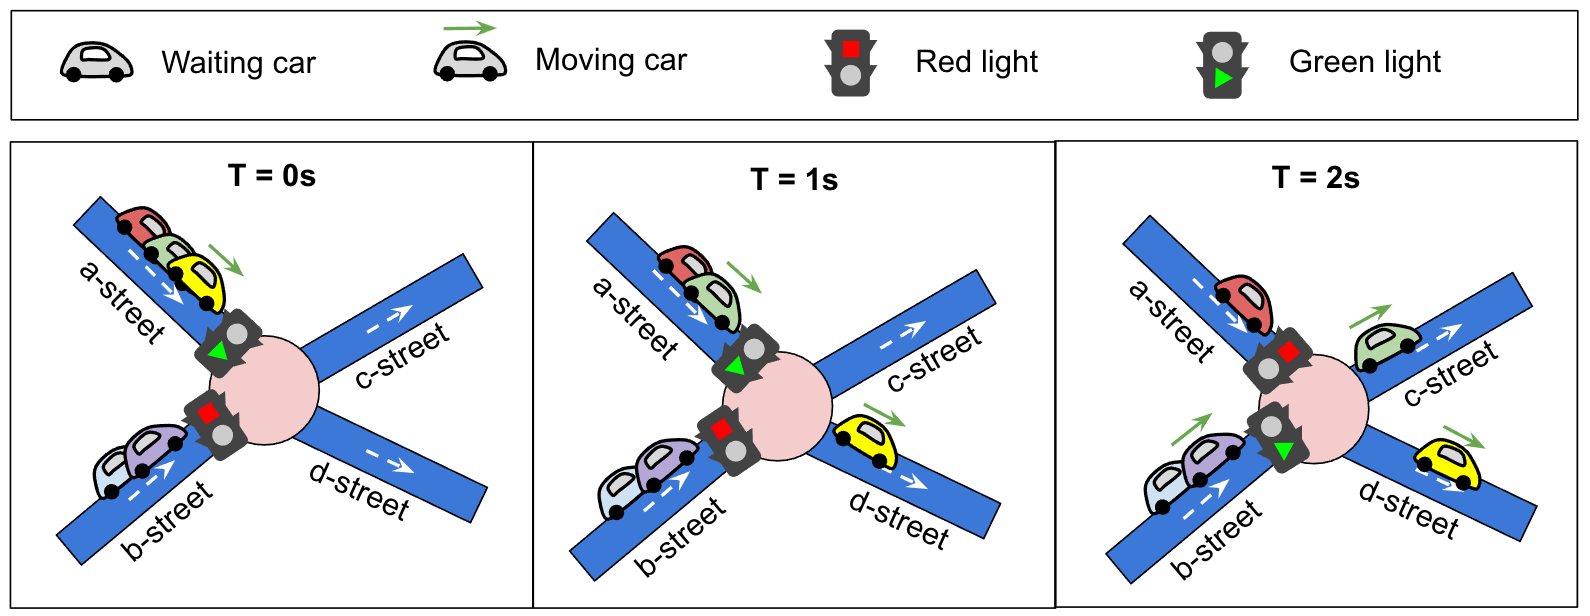
\includegraphics[width=\linewidth]{img/hashcode/figure2-abc.png}
    % 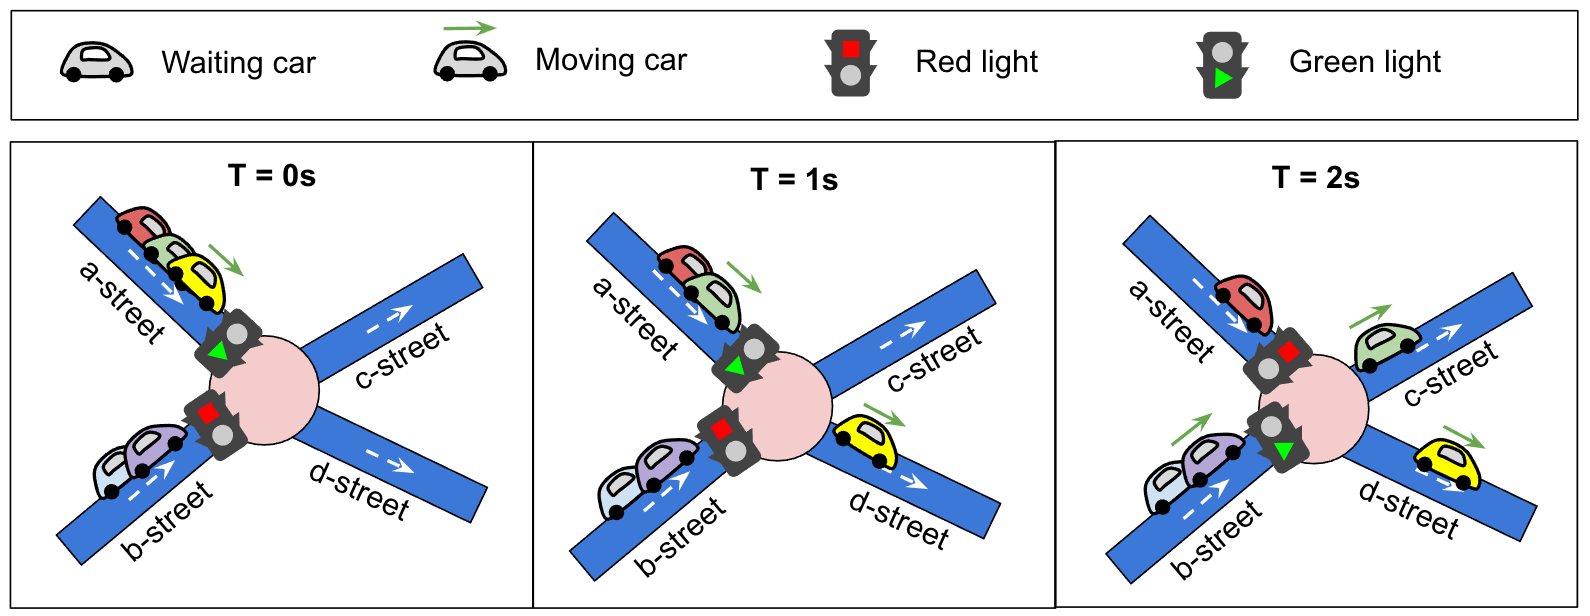
\includegraphics[width=.8\linewidth]{img/hashcode/figure2-abc.png}
    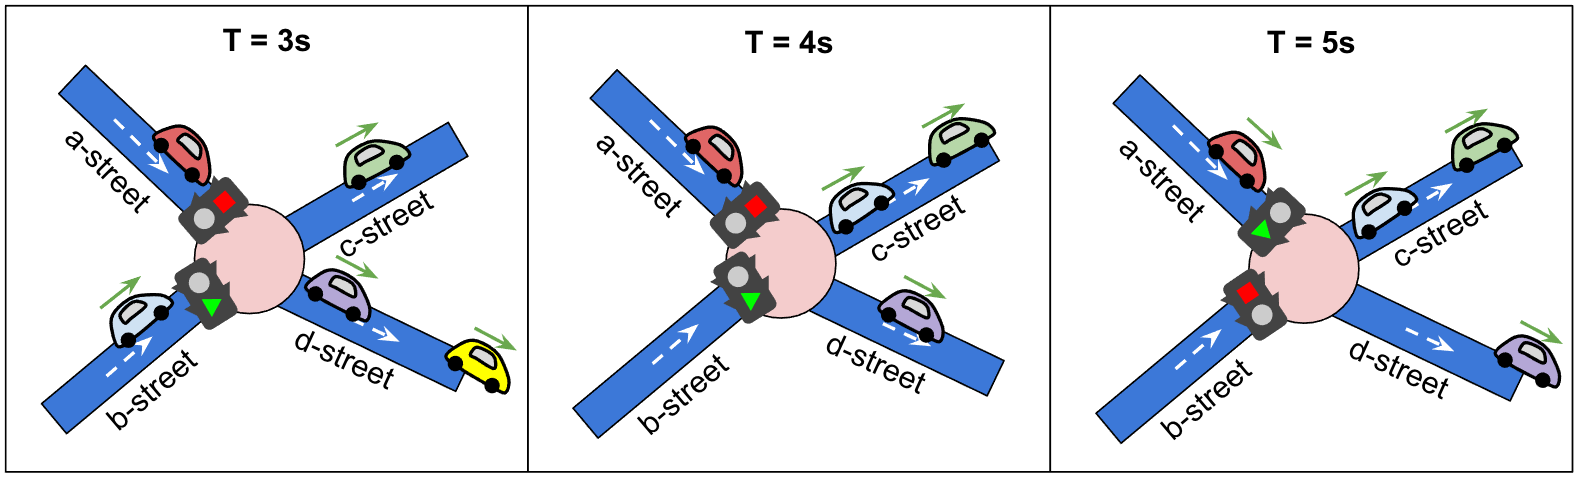
\includegraphics[width=\linewidth]{img/hashcode/figure2-def.png}
    % 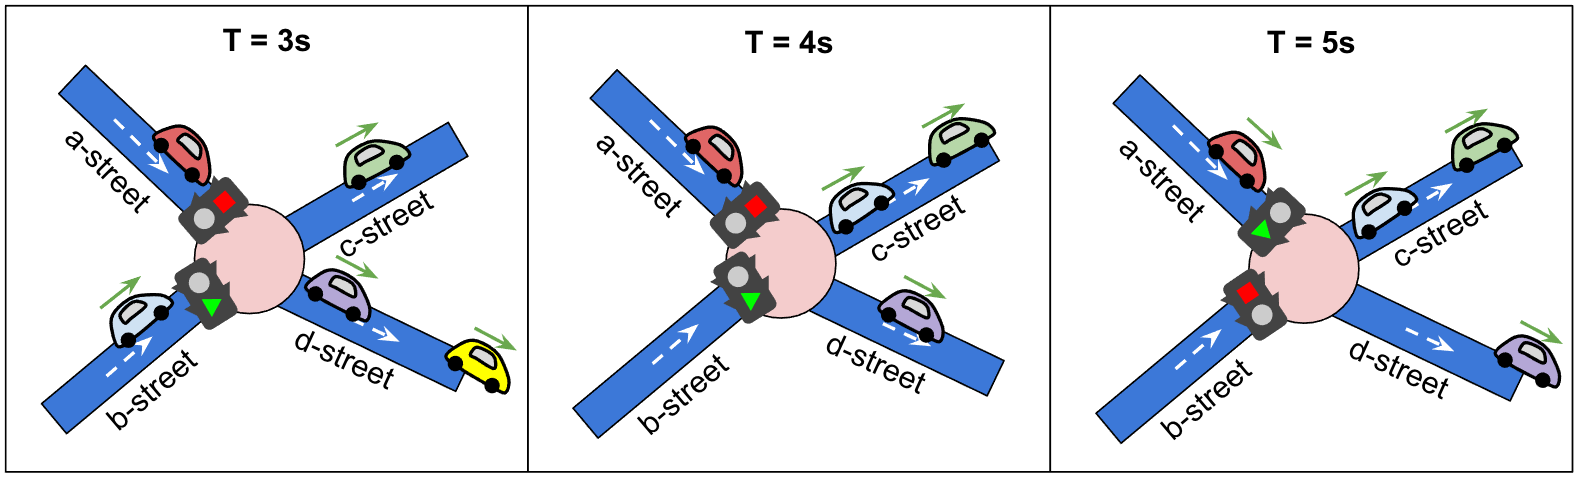
\includegraphics[width=.8\linewidth]{img/hashcode/figure2-def.png}
    \caption[Example of a traffic light schedule]{
        This figure shows how the traffic light schedule works for an intersection with two incoming streets \cite{google2023google}.
        The schedule is as follows: First \textit{a-street} for $2$ seconds, then \textit{b-street} for $3$ seconds.
        We can see the first two cars from \textit{a-street} pass in the first two seconds, then the green light switches to \textit{b-street} for three seconds,
        allowing the two cars from \textit{b-street} pass. The last car from \textit{a-street} waits till the beginning of the next cycle and then passes.
    }
    \label{fig:hashcode_traffic_lights}
\end{figure}

\subsection{Cars} \label{subsec:cars}

Furthermore, we have a set of cars $C$, where $\abs{C} \in [1, 10^3]$. Each car $c \in C$ has a given path $\bm{p_c}$ through the city. The path is a sequence of streets the car has to drive through.
The number of streets in each path $\bm{p_c}$ is in the range $[2, 10^3]$.
No intersection or street can be repeated in a path.

At the beginning of the simulation, all cars are at the end of the first street in their path. They either wait if the light is red or are ready to move if the light is green. If more cars start at the end of the same street, they queue up according to their IDs in the input file (see Figure~\ref{fig:hashcode_street}). When a car reaches the end of the last street in its path, it is immediately removed from the street.

\begin{figure}[ht] % h = here, t = top, p = page of floats
    \centering
    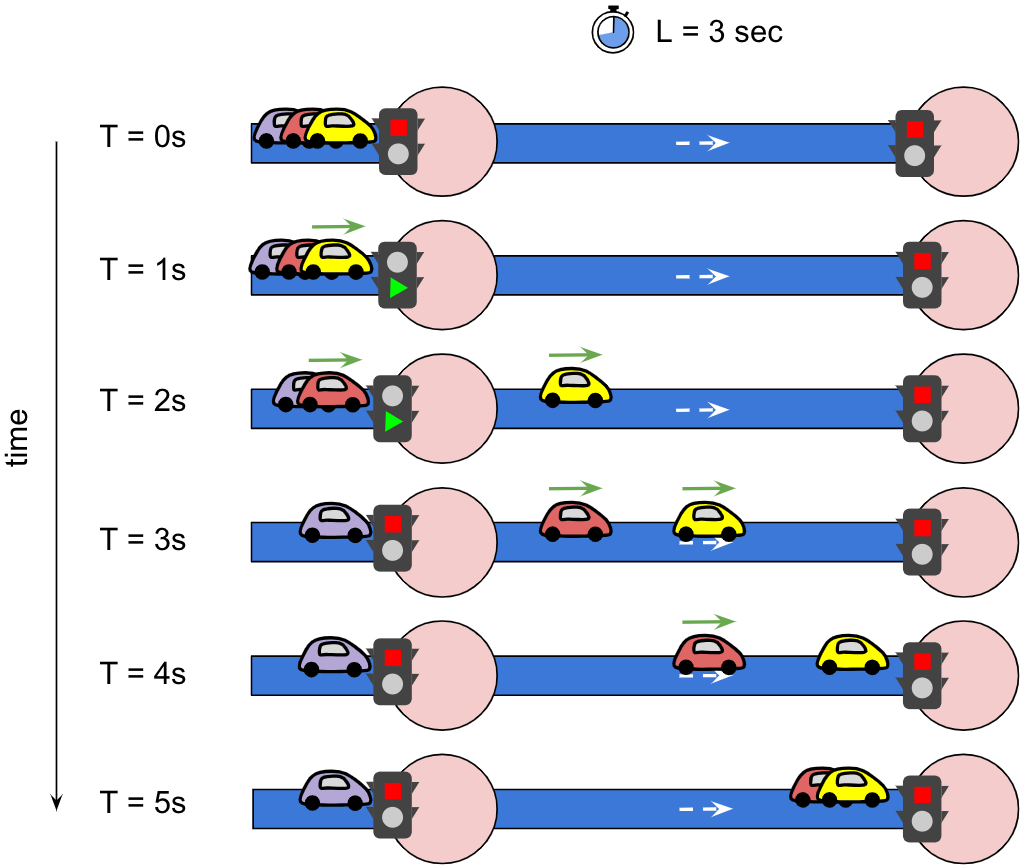
\includegraphics[width=\linewidth]{img/hashcode/figure3.png}
    %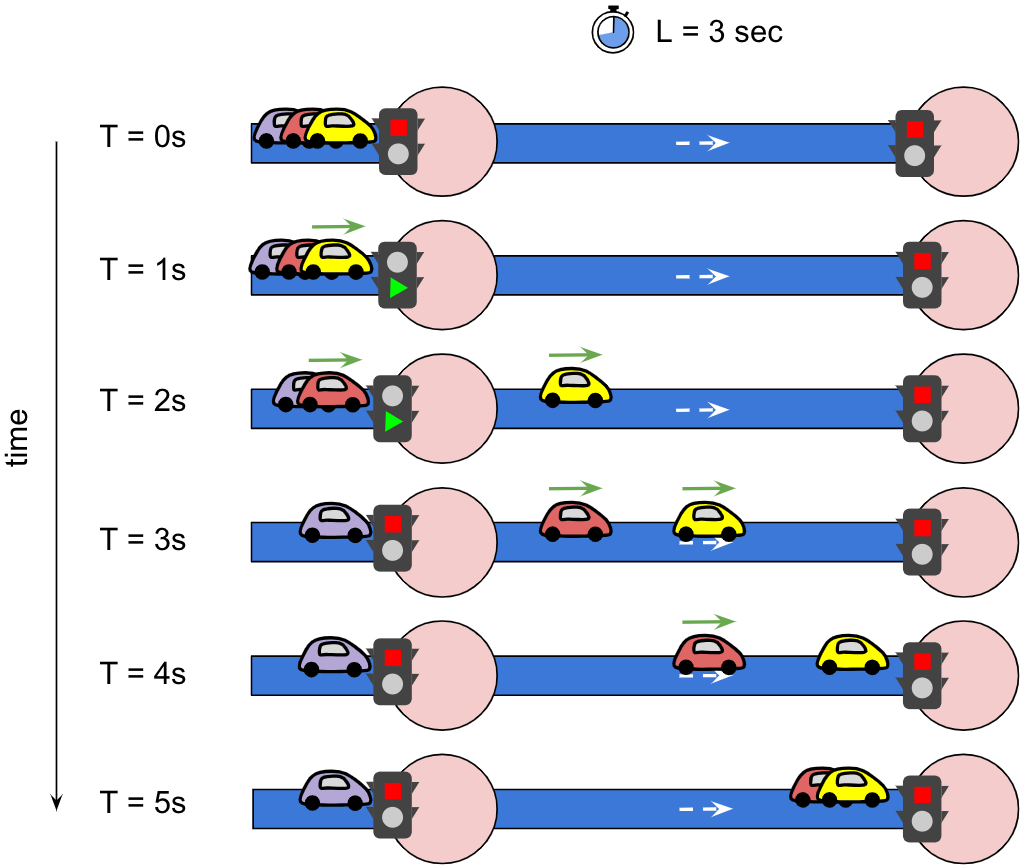
\includegraphics[width=.8\linewidth]{img/hashcode/figure3.png}
    \caption[Example of cars driving through a street]{
        This figure shows the first five seconds of a~simulation \cite{google2023google}.
        For simplicity, only one street is shown in the figure; when the light is red for this street, it is green for another street in the same intersection.
        When the light turns green at $T=1s$, the first (yellow) car immediately passes the intersection and moves to the next street, reaching the end of the street at $T=4s$.
        At $T=2s$, the light is still green, so the second (red) car passes the intersection and moves to the next street, reaching the end of the street at $T=5s$.
        From $T=3s$ to $T=5s$, the light is red, so the third (purple) car cannot pass the intersection and has to wait for the next cycle.
    }
    \label{fig:hashcode_street}
\end{figure}

\subsection{Score}

The score reflects the quality of the traffic light schedules: the more cars reach their destination, and the sooner they arrive, the higher the score.
The objective is to maximize this value.
In the context of optimization, the score serves as a \textit{fitness function}.

The score is determined as follows. Let $\bm{\theta}$ denote the traffic light schedules, and let $C$ be the set of cars.
Given a simulation duration $\mathrm{D} \in [1, 10^4]$ in seconds,
and a fixed bonus awarded for reaching the destination $\mathrm{F} \in [1, 10^3]$,
let $t(c; \bm{\theta}) \in \mathbb{N}$ be the time when a car $c \in C$ reaches its destination.
The score of a single car $c$ under the schedules $\bm{\theta}$ is defined as
\begin{equation}
    score(c; \bm{\theta}) =
    \begin{cases}
        \mathrm{F} + (\mathrm{D} - t(c; \bm{\theta})), & \text{if $t(c; \bm{\theta}) \leq \mathrm{D}$}, \\
        0, & \text{otherwise}.
    \end{cases}
\end{equation}
Then, the total score of the schedules $\bm{\theta}$ is defined as
\begin{equation}
    SCORE(\bm{\theta}) = \sum_{c \in C} score(c; \bm{\theta}).
\end{equation}

\section{Preprocessing of a problem instance} \label{sec:preprocessing}

In this section, we introduce preprocessing steps that we apply to reduce the total number of parameters we need to optimize.
These are our own observations and are not part of the original problem statement. After preprocessing, a substantial amount of intersections and streets is removed from optimization, which allows us to save resources and focus only on the important parameters. We also describe the format in which we represent the schedules.

\subsection{Preprocessing steps}
Throughout this section, we introduce some additional terms to help us better describe the steps.

\paragraph{Used and unused streets}
\textit{Unused street} is a street that is the final destination of all cars that have it in their path (i.e., a traffic light for this street is not needed).
\textit{Used street} is a street that is not the final destination of at least one car that has it in its path.

\paragraph{Used and unused intersections} \textit{Unused intersection} is an intersection where all incoming streets are unused streets. \textit{Used intersection} is an intersection with at least one used incoming street.

% https://tex.stackexchange.com/questions/32160/new-line-after-paragraph
\paragraph{Step 1: Remove unused intersections and unused streets} \label{para:step_1} \mbox{} \\
Remove unused intersections and unused incoming streets from used intersections. \\

\hyperref[para:step_1]{Step 1} is an obvious one; unused intersections are never used and only add unnecessary complexity. Unused incoming streets in used intersections prolong the traffic light cycle for the whole intersection, which very frequently leads to longer waiting times and thus a lower score. We now proceed to the next step.

\paragraph{Trivial and non-trivial intersections}
There are two types of used intersections: trivial and non-trivial.
\textit{Trivial intersection} is an intersection with exactly one used incoming street. \textit{Non-trivial intersection} is an intersection with two or more used incoming streets.

\paragraph{Trivial and non-trivial streets}
For completeness, we also split the used streets into trivial and non-trivial ones.
\textit{Trivial street} is a used incoming street in a trivial intersection. \textit{Non-trivial street} is a used incoming street in a non-trivial intersection.

\paragraph{Step 2: Fix the schedule for trivial intersections; optimize only schedules of non-trivial intersections} \label{para:step_2}
For each trivial intersection, the schedule can be fixed by assigning a green light to its only used incoming street for the entire duration. Trivial intersections can then be removed from optimization, and only schedules of non-trivial intersections are optimized. \\

Let us think about \hyperref[para:step_2]{Step 2} in more detail. For trivial intersections, we have two meaningful schedule options:
\begin{enumerate}
    \item Keep the light green the whole time.
    \item Keep the light red the whole time, effectively blocking all cars there.
\end{enumerate}
Empirically speaking, the vast majority of trivial intersections should be kept green, otherwise many cars would not be able to reach their destination at all.

However, suppose that keeping the light red for some trivial intersection improves the score. This means that there must be a problematic car passing through this intersection. Such a car must eventually reach some non-trivial intersection via a street, and this street can still be set to have a red light the whole time during optimization. We therefore leave this up to the optimization algorithm, hoping that it explores this option if it is indeed beneficial. \\

To demonstrate the usefulness of preprocessing, Tables~\ref{tab:intersection_statistics} and \ref{tab:street_statistics} show statistics of intersections and streets for each dataset. After applying both steps, we are only left with non-trivial intersections and non-trivial streets for optimization. This enables us to skip optimizing thousands of parameters.

% TABLE OF INTERSECTION STATISTICS
\begin{table}[h]
\centering\footnotesize\sf

\begin{tabular}{lr@{\hspace{0.1cm}}r@{\hspace{0.5cm}}r@{\hspace{0.1cm}}r@{\hspace{0.5cm}}r@{\hspace{0.1cm}}r}

& \multicolumn{6}{c}{\textbf{Intersections}} \\
\addlinespace[2pt]
\toprule
Dataset & \multicolumn{2}{c}{Unused} & \multicolumn{2}{c}{Trivial} & \multicolumn{2}{c}{Non-trivial} \\
\midrule
\textbf{A} & 1 & (25\%) & 2 & (50\%) & \textbf{1} & \textbf{(25\%)} \\
\textbf{B} & 777 & (11\%) & 4,977 & (70\%) & \textbf{1,319} & \textbf{(19\%)} \\
\textbf{C} & 2,340 & (23\%) & 4,468 & (45\%) & \textbf{3,192} & \textbf{(32\%)} \\
\textbf{D} & 0 & (0\%) & 0 & (0\%) & \textbf{8,000} & \textbf{(100\%)} \\
\textbf{E} & 0 & (0\%) & 263 & (53\%) & \textbf{237} & \textbf{(47\%)} \\
\textbf{F} & 30 & (2\%) & 332 & (20\%) & \textbf{1,300} & \textbf{(78\%)} \\
\bottomrule
\end{tabular}

\caption[Intersection statistics]{Intersection statistics across all datasets.}
\label{tab:intersection_statistics}
\end{table}

% TABLE OF STREET STATISTICS
\begin{table}[h]
\centering\footnotesize\sf

\begin{tabular}{lr@{\hspace{0.1cm}}r@{\hspace{0.5cm}}r@{\hspace{0.1cm}}r@{\hspace{0.5cm}}r@{\hspace{0.1cm}}r}

& \multicolumn{6}{c}{\textbf{Streets}} \\
\addlinespace[2pt]
\toprule
Dataset & \multicolumn{2}{c}{Unused} & \multicolumn{2}{c}{Trivial} & \multicolumn{2}{c}{Non-trivial} \\
\midrule
\textbf{A} & 1 & (20\%) & 2 & (40\%) & \textbf{2} & \textbf{(40\%)} \\
\textbf{B} & 1,138 & (12\%) & 4,977 & (55\%) & \textbf{2,987} & \textbf{(33\%)} \\
\textbf{C} & 23,558 & (67\%) & 4,468 & (13\%) & \textbf{7,004} & \textbf{(20\%)} \\
\textbf{D} & 12,054 & (13\%) & 0 & (0\%) & \textbf{83,874} & \textbf{(87\%)} \\
\textbf{E} & 42 & (4\%) & 263 & (26\%) & \textbf{693} & \textbf{(70\%)} \\
\textbf{F} & 4,667 & (47\%) & 332 & (3\%) & \textbf{5,001} & \textbf{(50\%)} \\
\bottomrule
\end{tabular}

\caption[Street statistics]{Street statistics across all datasets.}
\label{tab:street_statistics}
\end{table}

From now on, whenever we refer to schedules, we mean the \textit{schedules of non-trivial intersections with non-trivial streets}, as these intersections and streets are the only ones that are left after preprocessing.

\subsection{Schedules format} \label{subsec:schedules_format}

Each schedule of an intersection consists of two parts: \textit{order} and \textit{times}. Order is an array of street indices that defines the order in which the streets have the green light. Times is an array of integers that defines the duration of the green light with respect to the street order.
For illustration, recall the schedule from Figure~\ref{fig:hashcode_traffic_lights}; street-a (ID 0) has a green light for 2 seconds, and then street-b (ID~1) has a green light for 3 seconds. This schedule is represented in our format as follows:
\vspace{-0.4cm}
\begin{align*}
\text{Order} \quad& \text{Times} \\
\Big([0, 1], \quad& [2, 3]\Big).
\end{align*}
Then, the schedules are collectively represented as
\begin{quote}
    a \textbf{list of pairs}, where each pair consists of \textbf{order} and \textbf{times} arrays.
\end{quote}

\section{Datasets} \label{sec:datasets}

This section briefly describes all datasets provided with the problem.
The datasets vary in the size and structure of their city plans.
In the previous section, we already showed statistics of intersections and streets (see Tables~\ref{tab:intersection_statistics} and \ref{tab:street_statistics}).
Here we compare the datasets by the number of parameters we need to optimize.
That is, twice the number of non-trivial streets---one parameter for the order and one for the time. Note that this is only one way to compare the datasets, and it does not account for the actual paths cars must take or how convoluted those paths may be.

\begin{figure}[h]
    \centering
    % 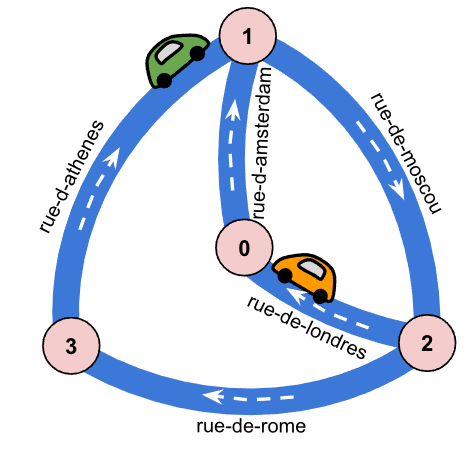
\includegraphics[width=\linewidth]{img/hashcode/figure5.png}
    % 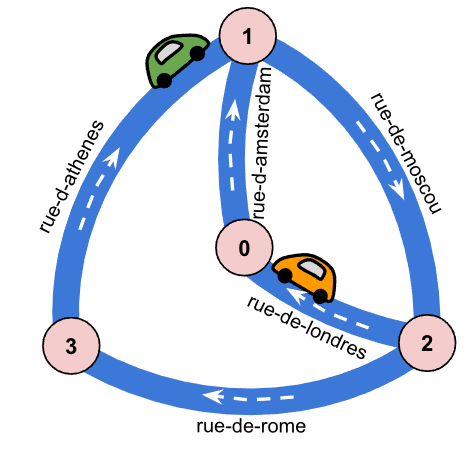
\includegraphics[width=.6\linewidth]{img/hashcode/figure5.png}
    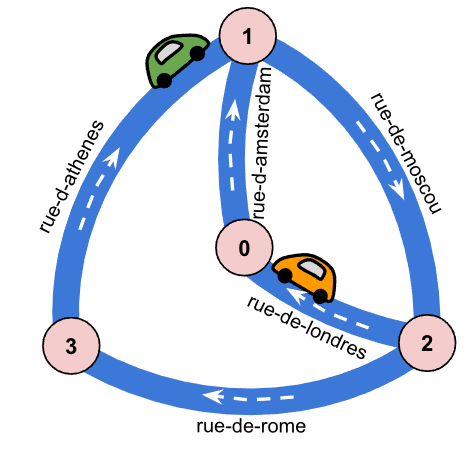
\includegraphics[width=.5\linewidth]{img/hashcode/figure5.png}
    \caption[Visualization of dataset A]{
        Visualization of dataset A \cite{google2023google}.
    }
    \label{fig:hashcode_dataset_a}
\end{figure}

\paragraph{A - An example: 4 parameters} Simple toy problem dataset used for debugging (see Figure~\ref{fig:hashcode_dataset_a}).

\paragraph{B - By the ocean: 5,974 parameters} Dataset based on a real city plan of Lisbon, Portugal (see Figure~\ref{fig:hashcode_dataset_b}).

\begin{figure}[h]
    \centering
    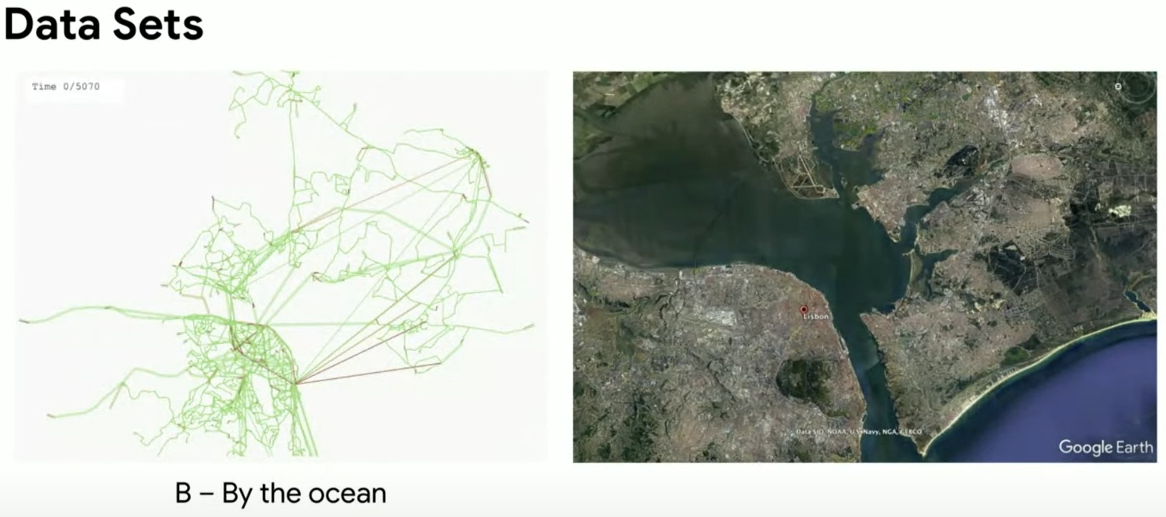
\includegraphics[width=\linewidth]{img/screenshots/hashcode_datasets_b.png}
    % 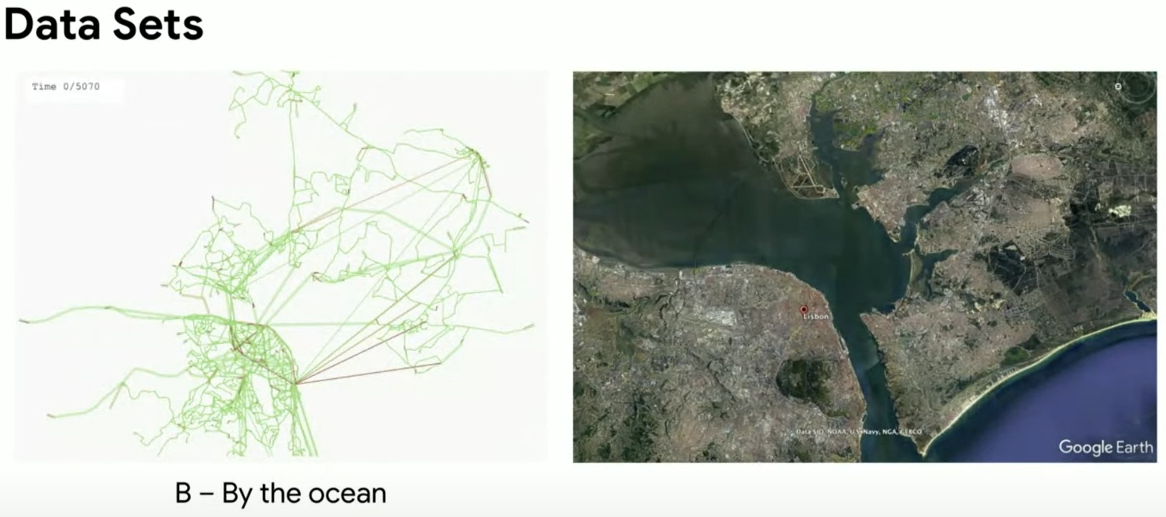
\includegraphics[width=.8\linewidth]{img/screenshots/hashcode_datasets_b.png}
    \caption[Visualization of dataset B]{
        Dataset B based on the real data of Lisbon on the right. Screenshot from \href{https://www.youtube.com/watch?v=YPOVd-hQUjA}{Hash Code 2021: Online Qualification Round Livestream}.
    }
    \label{fig:hashcode_dataset_b}
\end{figure}

\paragraph{C - Checkmate: 14,008 parameters} Dataset with a chessboard-like pattern and regular structure of intersections and streets (see Figure~\ref{fig:hashcode_dataset_c_e}).

% https://codeforces.com/blog/entry/88188#comment-765574
\paragraph{D - Daily commute: 167,748 parameters} By far the largest dataset with a challenging-to-navigate network from the \textit{Barabási-Albert} distribution \cite{albert2002statistical}.

\paragraph{E - Etoile: 1,386 parameters} Nicknamed \textit{Etoile}\footnote{\textit{Étoile} means star in French.}, this dataset is a one big star, meaning there is one very important intersection in the middle with hundreds of incoming streets (see Figure~\ref{fig:hashcode_dataset_c_e}).

\paragraph{F - Forever jammed: 10,002 parameters} Medium sized dataset but again with a complex network difficult to optimize.

\begin{figure}[h]
    \centering
    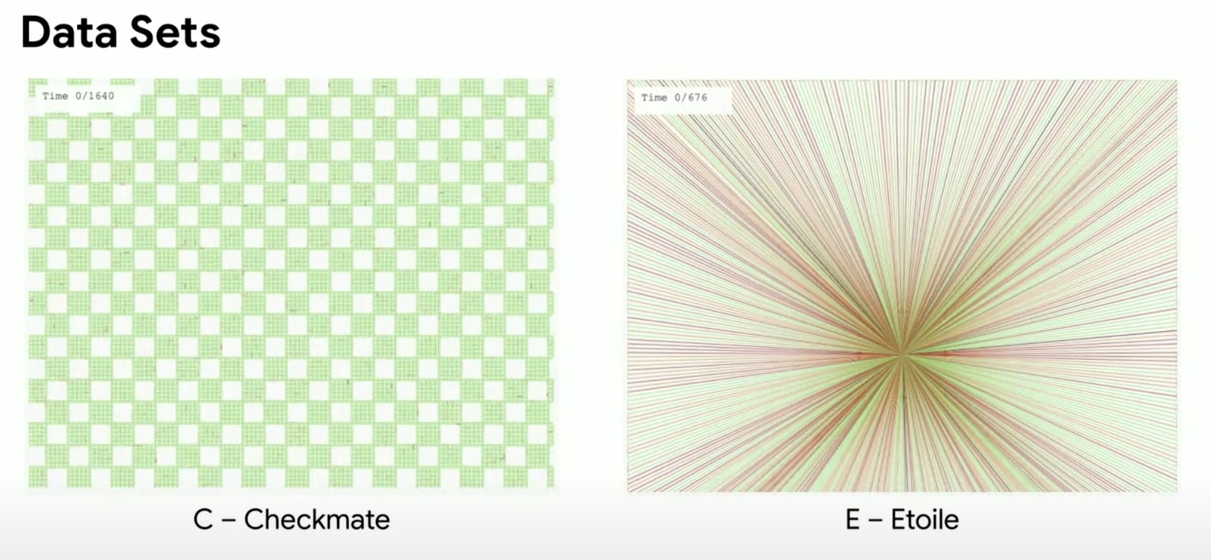
\includegraphics[width=\linewidth]{img/screenshots/hashcode_datasets_c_e.png}
    % 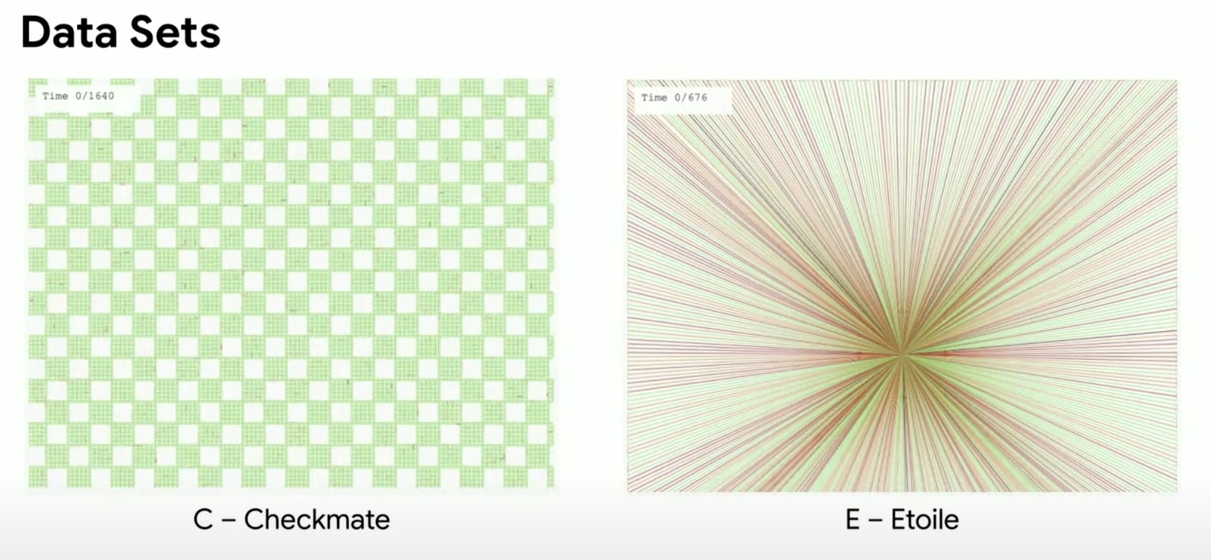
\includegraphics[width=.8\linewidth]{img/screenshots/hashcode_datasets_c_e.png}
    \caption[Visualization of datasets C and E]{
        Visualization of datasets C and E. Screenshot from \href{https://www.youtube.com/watch?v=YPOVd-hQUjA}{Hash Code 2021: Online Qualification Round Livestream}.
    }
    \label{fig:hashcode_dataset_c_e}
    \end{figure}

\subsection{Score normalization} \label{subsec:score_normalization}

As mentioned in Section~\ref{sec:competition_overview}, each dataset yields an absolute score within a different range. To compare the performance across all datasets, we normalize the scores to a 0--1 scale, where 0 represents our baseline solution (see Section~\ref{sec:initial_schedules} for details), and 1 corresponds to the maximum known score\footnote{See the maximum known scores at \\\url{https://github.com/sagishporer/hashcode-2021-qualification\#score}.} for the dataset. Note that the baseline is already a good solution, so there may be limited room for improvement---for example, in dataset B.

\section{Simulator} \label{sec:simulator}

This section provides a brief overview of the custom simulator that we developed to serve as a black-box fitness function for the optimization algorithms. We discuss the motivation behind its design and describe the functionality relevant to the optimization process.
For further information on using the simulator or regarding its implementation, please refer to the user guide in Appendix~\ref{chap:user_guide} and the developer documentation in Appendix~\ref{chap:developer_documentation}.

\medskip

Our simulator replaces the original competition evaluation system, which was accessible only through the competition website via a user interface and is no longer available. It also adds several features on top of the original system.
The simulator is written in C++ to be as fast and efficient as possible, and is wrapped as a Python package using the powerful pybind11 library~\cite{jakob2017pybind11}, making it very convenient to use.
Inspired by libraries such as NumPy\footnote{\url{https://numpy.org/}} and PyTorch\footnote{\url{https://pytorch.org/}}, our goal is to provide an easy-to-use interface and seamless integration with the vital Python ecosystem, without compromising on top-tier performance.

Following are the features of the simulator package that are important for optimization. These features are implemented in C++ and exposed through a lightweight Python API:
\begin{itemize}
    \item Reading and storing the input data.
    \item Creating initial schedules using several different options listed in Section~\ref{sec:initial_schedules}.
    \item Running the simulation to evaluate given schedules.
    \item Retrieving and updating schedules in a format described in Section~\ref{subsec:schedules_format}.
\end{itemize}

The only case where larger data are passed between C++ and Python is when retrieving and updating the schedules.
Since the optimization loop is implemented in Python using parts of the DEAP library~\cite{fortin2012deap}, it must retrieve the schedules from the simulator, modify them externally, and then send them back into the simulator to evaluate their score.
